Zunächst werden der Acrylblock und die Lage der Fehlstellen mittels Schieblehre
bestimmt. Der Block hat eine Höhe von $h=8.07\cm$ und eine Länge von $l=15\cm$.
In Tabelle \ref{tab:oben} sind die Orte der Fehlstellen mit Schieblehre, A-Scan
und B-Scan aufgeführt. Die erste Messung wurde so durchgeführt, dass die Bohrung
11 im unteren Teil des Blocks \ref{fig:block} lokalisiert ist. Der A-Scan wurde
mit einer $1\MHz$- und der B-Scan mit einer $2\MHz$-Sonde durchgeführt.
\begin{table}[H]
  \centering
  \begin{tabular}{cc|cc|cc}
    \toprule
    \multicolumn{1}{c}{Loch}& \multicolumn{1}{c|}{Schieblehre} & \multicolumn{2}{c|}{A-Scan}
    & \multicolumn{2}{c}{B-Scan} \\
    & $t/\ms$ & $s\cm$ & $t/\ms$ & $s/\cm$ & $s/\cm$ \\
    \midrule
     1  &  1.8 &  17.7 & 2.4 & 15.3 & 2.1 \\
     2  &  1.7 &  15.3 & 2.1 & 14.2 & 1.9 \\
     3  &  7.1 &  46.0 & 6.3 & 45.7 & 6.2 \\
     4  &  6.3 &  40.7 & 5.6 & 40.3 & 5.5 \\
     5  &  5.5 &  35.3 & 4.8 & 35.0 & 4.8 \\
     6  &  4.7 &  29.8 & 4.1 & 29.5 & 4.0 \\
     7  &  3.9 &  24.0 & 3.3 & 23.7 & 3.2 \\
     8  &  3.0 &  18.2 & 2.5 & 17.9 & 2.4 \\
     9  &  2.2 &  12.4 & 1.7 & 12.2 & 1.7 \\
    10  &  1.3 &   6.7 & 0.9 &  6.6 & 0.9 \\
    11  &  5.6 &  42.0 & 5.7 & 41.9 & 5.7 \\
    \bottomrule
  \end{tabular}
  \caption{Lage der Bohrungen von oben.}
  \label{tab:oben}
\end{table}
Danach wurde die Messung erneut durchgeführt, der Block wird jedoch so gedreht,
dass sich Bohrung 11 im oberen Teil des Blocks \ref{fig:block} befindet.
Die Werte für diese Messung sind in Tabelle \ref{tab:unten} zu sehen.
\begin{table}[H]
  \centering
  \begin{tabular}{cc|cc|cc}
    \toprule
    \multicolumn{1}{c}{Loch}& \multicolumn{1}{c|}{Schieblehre} & \multicolumn{2}{c|}{A-Scan}
    & \multicolumn{2}{c}{B-Scan} \\
    & $t/\ms$ & $s\cm$ & $t/\ms$ & $s/\cm$ & $s/\cm$ \\
    \midrule
     1  &   6.0 &  45.0 & 6.1 & 45.2 & 6.2 \\
     2  &   6.2 &  48.0 & 6.6 & 46.2 & 6.3 \\
     3  &   1.3 &  11.3 & 1.5 & 11.1 & 1.5 \\
     4  &   2.2 &  17.3 & 2.4 & 17.0 & 2.3 \\
     5  &   3.0 &  23.6 & 3.2 & 23.1 & 3.1 \\
     6  &   3.9 &  29.9 & 4.1 & 29.5 & 4.0 \\
     7  &   4.7 &  35.6 & 4.9 & 35.2 & 4.8 \\
     8  &   5.5 &  41.3 & 5.6 & 41.1 & 5.6 \\
     9  &   6.3 &  47.1 & 6.4 & 47.0 & 6.4 \\
    10  &   7.1 &  53.5 & 7.3 & \hrulefill & \hrulefill \\
    11  &   1.6 &  12.7 & 1.7 & 12.4 & 1.7 \\
    \bottomrule
  \end{tabular}
  \caption{Lage der Bohrungen von oben.}
  \label{tab:unten}
\end{table}
Die Aufnahmebilder des B-Scans sind in Abbildung \ref{fig:bscan} zu sehen.
\begin{figure}[H]
  \centering
  \begin{subfigure}{0.4\textwidth}
    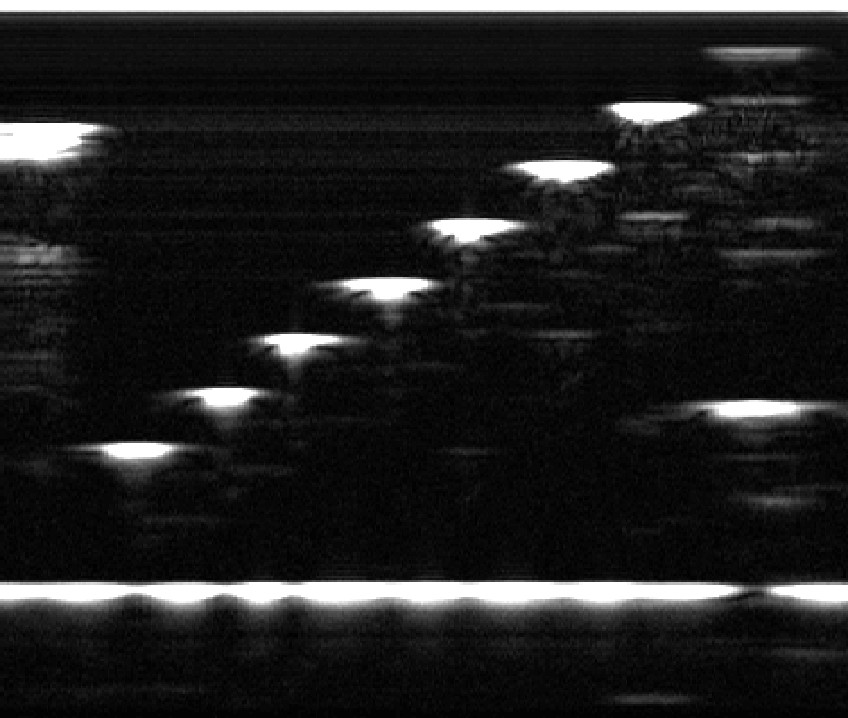
\includegraphics[width=6cm]{bilder/B-ScanUnten.jpg}
    \caption{B-Scan von Oben}
    \label{sub:oben}
  \end{subfigure}
  \begin{subfigure}{0.4\textwidth}
  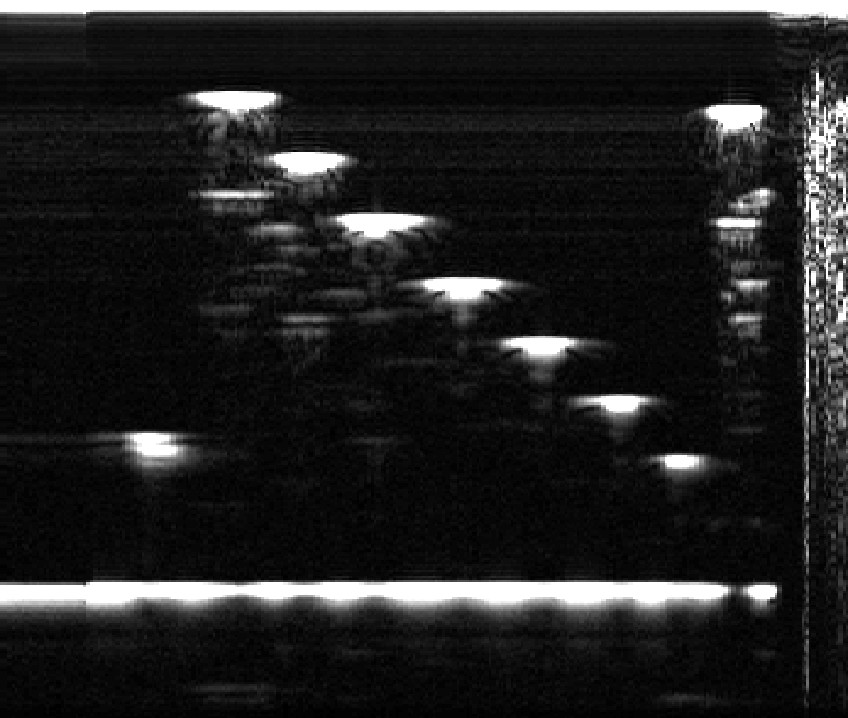
\includegraphics[width=6cm]{bilder/B-ScanOben.jpg}
  \caption{B-Scan von Unten}
  \label{sub:unten}
\end{subfigure}
\caption{Aufnahmebilder des B-Scans}
\label{fig:bscan}
\end{figure}
Hieraus lassen sich die Durchmesser der einzelnen Bohrungen bestimmen, indem
die gemessenen Abstände der Fehlstellen zum Blockrand von der Gesamtblockhöhe
subtrahiert werden. Die einzelenen Durchmesser sind in der untenstehenden
Tabelle \ref{tab:durch} aufgeführt.
\begin{table}[H]
  \centering
  \begin{tabular}{cccc}
    \toprule
    \multicolumn{1}{c}{Loch}&\multicolumn{1}{c}{Schieblehre}&
    \multicolumn{1}{c}{A-Scan}&\multicolumn{1}{c}{B-Scan} \\
    Nummer & $d/\cm$ & $d/\cm$ & $d/\cm$ \\
    \midrule
     1 & 0.26 & -0.37  &  -0.07      \\
     2 & 0.17 & -0.45  &  -0.05      \\
     3 & 0.62 &  0.37  &   0.44      \\
     4 & 0.52 &  0.27  &   0.37      \\
     5 & 0.43 &  0.15  &   0.26      \\
     6 & 0.33 &  0.04  &   0.14      \\
     7 & 0.33 &  0.05  &   0.15      \\
     8 & 0.24 &  0.07  &   0.14      \\
     9 & 0.32 &  0.07  &   0.11      \\
    10 & 0.25 & -0.03  &  \hrulefill \\
    11 & 0.96 &  0.72  &   0.78      \\
    \bottomrule
  \end{tabular}
  \caption{Durchmesser der Fehlstellen}
  \label{tab:durch}
\end{table}
Nun wird das Auflösungsverfahren einer $1\MHz$-Sonde mittels A-Scan mit dem
Auflösungsvermögen einer $2\MHz$-Sonde verglichen. Hierfür wird erneut der
Durchmesser für die Löcher 1 und 2 bestimmt.
\begin{table}
  \begin{tabular}{ccc}
    \centering
    \toprule
    \multicolumn{1}{c}{Sonde}&\multicolumn{2}{c}{Durchmesser}\\
    $\nu/\MHz$ & $d_1/\cm$ & $d_2/\cm$ \\
    \midrule
    1  &  -0.37  &  -0.45 \\
    2  &   0.19  &   0.22 \\
    \bottomrule
  \end{tabular}
  \caption{Auflösungsvermögen verschiedener Sonden}
  \label{tab:auf}
\end{table}
